\documentclass[]{article}
\usepackage{lmodern}
\usepackage{amssymb,amsmath}
\usepackage{ifxetex,ifluatex}
\usepackage{fixltx2e} % provides \textsubscript
\ifnum 0\ifxetex 1\fi\ifluatex 1\fi=0 % if pdftex
  \usepackage[T1]{fontenc}
  \usepackage[utf8]{inputenc}
\else % if luatex or xelatex
  \ifxetex
    \usepackage{mathspec}
  \else
    \usepackage{fontspec}
  \fi
  \defaultfontfeatures{Ligatures=TeX,Scale=MatchLowercase}
\fi
% use upquote if available, for straight quotes in verbatim environments
\IfFileExists{upquote.sty}{\usepackage{upquote}}{}
% use microtype if available
\IfFileExists{microtype.sty}{%
\usepackage{microtype}
\UseMicrotypeSet[protrusion]{basicmath} % disable protrusion for tt fonts
}{}
\usepackage[margin=1in]{geometry}
\usepackage{hyperref}
\hypersetup{unicode=true,
            pdftitle={Code Generalization},
            pdfauthor={Asha Goodman},
            pdfborder={0 0 0},
            breaklinks=true}
\urlstyle{same}  % don't use monospace font for urls
\usepackage{color}
\usepackage{fancyvrb}
\newcommand{\VerbBar}{|}
\newcommand{\VERB}{\Verb[commandchars=\\\{\}]}
\DefineVerbatimEnvironment{Highlighting}{Verbatim}{commandchars=\\\{\}}
% Add ',fontsize=\small' for more characters per line
\usepackage{framed}
\definecolor{shadecolor}{RGB}{248,248,248}
\newenvironment{Shaded}{\begin{snugshade}}{\end{snugshade}}
\newcommand{\KeywordTok}[1]{\textcolor[rgb]{0.13,0.29,0.53}{\textbf{#1}}}
\newcommand{\DataTypeTok}[1]{\textcolor[rgb]{0.13,0.29,0.53}{#1}}
\newcommand{\DecValTok}[1]{\textcolor[rgb]{0.00,0.00,0.81}{#1}}
\newcommand{\BaseNTok}[1]{\textcolor[rgb]{0.00,0.00,0.81}{#1}}
\newcommand{\FloatTok}[1]{\textcolor[rgb]{0.00,0.00,0.81}{#1}}
\newcommand{\ConstantTok}[1]{\textcolor[rgb]{0.00,0.00,0.00}{#1}}
\newcommand{\CharTok}[1]{\textcolor[rgb]{0.31,0.60,0.02}{#1}}
\newcommand{\SpecialCharTok}[1]{\textcolor[rgb]{0.00,0.00,0.00}{#1}}
\newcommand{\StringTok}[1]{\textcolor[rgb]{0.31,0.60,0.02}{#1}}
\newcommand{\VerbatimStringTok}[1]{\textcolor[rgb]{0.31,0.60,0.02}{#1}}
\newcommand{\SpecialStringTok}[1]{\textcolor[rgb]{0.31,0.60,0.02}{#1}}
\newcommand{\ImportTok}[1]{#1}
\newcommand{\CommentTok}[1]{\textcolor[rgb]{0.56,0.35,0.01}{\textit{#1}}}
\newcommand{\DocumentationTok}[1]{\textcolor[rgb]{0.56,0.35,0.01}{\textbf{\textit{#1}}}}
\newcommand{\AnnotationTok}[1]{\textcolor[rgb]{0.56,0.35,0.01}{\textbf{\textit{#1}}}}
\newcommand{\CommentVarTok}[1]{\textcolor[rgb]{0.56,0.35,0.01}{\textbf{\textit{#1}}}}
\newcommand{\OtherTok}[1]{\textcolor[rgb]{0.56,0.35,0.01}{#1}}
\newcommand{\FunctionTok}[1]{\textcolor[rgb]{0.00,0.00,0.00}{#1}}
\newcommand{\VariableTok}[1]{\textcolor[rgb]{0.00,0.00,0.00}{#1}}
\newcommand{\ControlFlowTok}[1]{\textcolor[rgb]{0.13,0.29,0.53}{\textbf{#1}}}
\newcommand{\OperatorTok}[1]{\textcolor[rgb]{0.81,0.36,0.00}{\textbf{#1}}}
\newcommand{\BuiltInTok}[1]{#1}
\newcommand{\ExtensionTok}[1]{#1}
\newcommand{\PreprocessorTok}[1]{\textcolor[rgb]{0.56,0.35,0.01}{\textit{#1}}}
\newcommand{\AttributeTok}[1]{\textcolor[rgb]{0.77,0.63,0.00}{#1}}
\newcommand{\RegionMarkerTok}[1]{#1}
\newcommand{\InformationTok}[1]{\textcolor[rgb]{0.56,0.35,0.01}{\textbf{\textit{#1}}}}
\newcommand{\WarningTok}[1]{\textcolor[rgb]{0.56,0.35,0.01}{\textbf{\textit{#1}}}}
\newcommand{\AlertTok}[1]{\textcolor[rgb]{0.94,0.16,0.16}{#1}}
\newcommand{\ErrorTok}[1]{\textcolor[rgb]{0.64,0.00,0.00}{\textbf{#1}}}
\newcommand{\NormalTok}[1]{#1}
\usepackage{graphicx,grffile}
\makeatletter
\def\maxwidth{\ifdim\Gin@nat@width>\linewidth\linewidth\else\Gin@nat@width\fi}
\def\maxheight{\ifdim\Gin@nat@height>\textheight\textheight\else\Gin@nat@height\fi}
\makeatother
% Scale images if necessary, so that they will not overflow the page
% margins by default, and it is still possible to overwrite the defaults
% using explicit options in \includegraphics[width, height, ...]{}
\setkeys{Gin}{width=\maxwidth,height=\maxheight,keepaspectratio}
\IfFileExists{parskip.sty}{%
\usepackage{parskip}
}{% else
\setlength{\parindent}{0pt}
\setlength{\parskip}{6pt plus 2pt minus 1pt}
}
\setlength{\emergencystretch}{3em}  % prevent overfull lines
\providecommand{\tightlist}{%
  \setlength{\itemsep}{0pt}\setlength{\parskip}{0pt}}
\setcounter{secnumdepth}{0}
% Redefines (sub)paragraphs to behave more like sections
\ifx\paragraph\undefined\else
\let\oldparagraph\paragraph
\renewcommand{\paragraph}[1]{\oldparagraph{#1}\mbox{}}
\fi
\ifx\subparagraph\undefined\else
\let\oldsubparagraph\subparagraph
\renewcommand{\subparagraph}[1]{\oldsubparagraph{#1}\mbox{}}
\fi

%%% Use protect on footnotes to avoid problems with footnotes in titles
\let\rmarkdownfootnote\footnote%
\def\footnote{\protect\rmarkdownfootnote}

%%% Change title format to be more compact
\usepackage{titling}

% Create subtitle command for use in maketitle
\newcommand{\subtitle}[1]{
  \posttitle{
    \begin{center}\large#1\end{center}
    }
}

\setlength{\droptitle}{-2em}

  \title{Code Generalization}
    \pretitle{\vspace{\droptitle}\centering\huge}
  \posttitle{\par}
    \author{Asha Goodman}
    \preauthor{\centering\large\emph}
  \postauthor{\par}
      \predate{\centering\large\emph}
  \postdate{\par}
    \date{1/29/2019}


\begin{document}
\maketitle

\section{Can you improve this analysis
code?}\label{can-you-improve-this-analysis-code}

\begin{Shaded}
\begin{Highlighting}[]
\KeywordTok{library}\NormalTok{(bio3d)}
\NormalTok{Test <-}\StringTok{ }\KeywordTok{read.pdb}\NormalTok{(}\StringTok{"4AKE"}\NormalTok{) }
\end{Highlighting}
\end{Shaded}

\begin{verbatim}
##   Note: Accessing on-line PDB file
\end{verbatim}

\begin{Shaded}
\begin{Highlighting}[]
\NormalTok{Control <-}\StringTok{ }\KeywordTok{read.pdb}\NormalTok{(}\StringTok{"1AKE"}\NormalTok{) }
\end{Highlighting}
\end{Shaded}

\begin{verbatim}
##   Note: Accessing on-line PDB file
##    PDB has ALT records, taking A only, rm.alt=TRUE
\end{verbatim}

\begin{Shaded}
\begin{Highlighting}[]
\NormalTok{Test2 <-}\StringTok{ }\KeywordTok{read.pdb}\NormalTok{(}\StringTok{"1E4Y"}\NormalTok{) }
\end{Highlighting}
\end{Shaded}

\begin{verbatim}
##   Note: Accessing on-line PDB file
\end{verbatim}

\begin{Shaded}
\begin{Highlighting}[]
\NormalTok{Test.chainA <-}\StringTok{ }\KeywordTok{trim.pdb}\NormalTok{(Test, }\DataTypeTok{chain=}\StringTok{"A"}\NormalTok{, }\DataTypeTok{elety=}\StringTok{"CA"}\NormalTok{)}
\NormalTok{Control.chainA <-}\StringTok{ }\KeywordTok{trim.pdb}\NormalTok{(Control, }\DataTypeTok{chain=}\StringTok{"A"}\NormalTok{, }\DataTypeTok{elety=}\StringTok{"CA"}\NormalTok{)}
\NormalTok{Test2.chainA <-}\StringTok{ }\KeywordTok{trim.pdb}\NormalTok{(Test2, }\DataTypeTok{chain=}\StringTok{"A"}\NormalTok{, }\DataTypeTok{elety=}\StringTok{"CA"}\NormalTok{)}
\NormalTok{Test.b <-}\StringTok{ }\NormalTok{Test.chainA}\OperatorTok{$}\NormalTok{atom}\OperatorTok{$}\NormalTok{b}
\NormalTok{Control.b <-}\StringTok{ }\NormalTok{Control.chainA}\OperatorTok{$}\NormalTok{atom}\OperatorTok{$}\NormalTok{b}
\NormalTok{Test2.b <-}\StringTok{ }\NormalTok{Test2.chainA}\OperatorTok{$}\NormalTok{atom}\OperatorTok{$}\NormalTok{b}
\KeywordTok{plotb3}\NormalTok{(Test.b, }\DataTypeTok{sse=}\NormalTok{Test.chainA, }\DataTypeTok{typ=}\StringTok{"l"}\NormalTok{, }\DataTypeTok{ylab=}\StringTok{"Bfactor"}\NormalTok{)}
\end{Highlighting}
\end{Shaded}

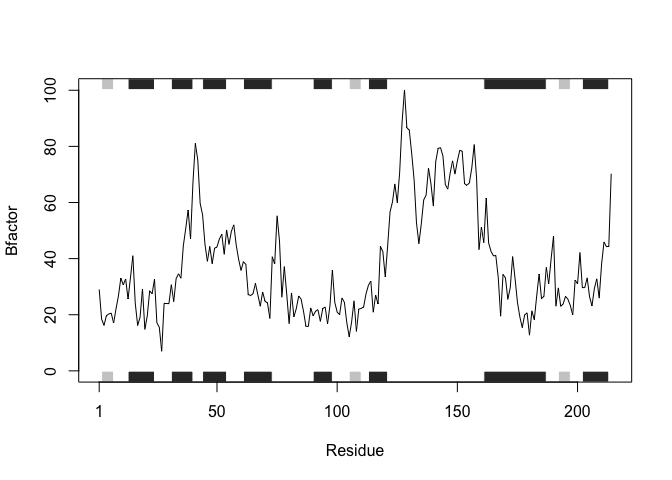
\includegraphics{Code_Generalization_files/figure-latex/unnamed-chunk-1-1.pdf}

\begin{Shaded}
\begin{Highlighting}[]
\KeywordTok{plotb3}\NormalTok{(Control.b, }\DataTypeTok{sse=}\NormalTok{Control.chainA, }\DataTypeTok{typ=}\StringTok{"l"}\NormalTok{, }\DataTypeTok{ylab=}\StringTok{"Bfactor"}\NormalTok{)}
\end{Highlighting}
\end{Shaded}

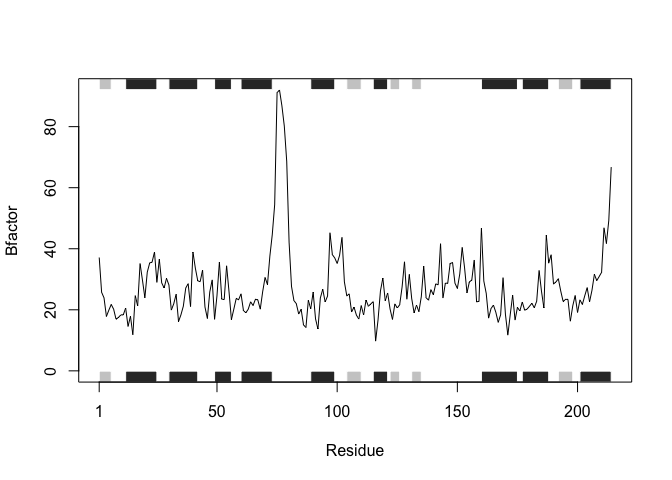
\includegraphics{Code_Generalization_files/figure-latex/unnamed-chunk-1-2.pdf}

\begin{Shaded}
\begin{Highlighting}[]
\KeywordTok{plotb3}\NormalTok{(Test2.b, }\DataTypeTok{sse=}\NormalTok{Test2.chainA, }\DataTypeTok{typ=}\StringTok{"l"}\NormalTok{, }\DataTypeTok{ylab=}\StringTok{"Bfactor"}\NormalTok{)}
\end{Highlighting}
\end{Shaded}

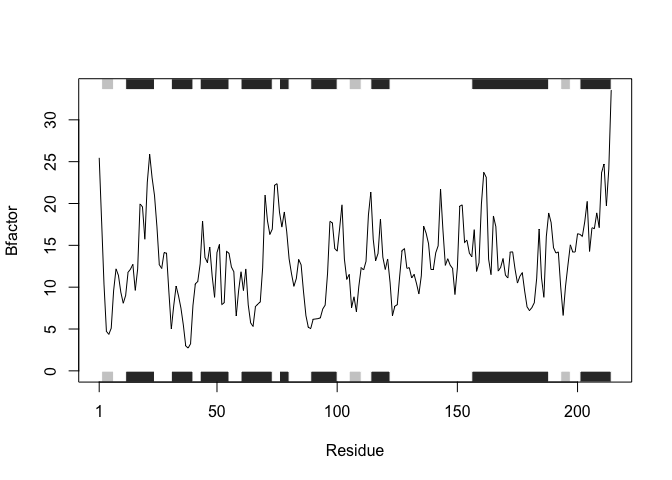
\includegraphics{Code_Generalization_files/figure-latex/unnamed-chunk-1-3.pdf}

\paragraph{\texorpdfstring{Answered simply, yes we can. Note we have now
made a new function that encompasses the previous functions that
\textbf{R}eads \textbf{a}nd \textbf{P}lots a \textbf{pdb for me} or
``rap\_pdb\_forme''. This function takes advantage of vectors and their
isolation in the function. For example, although we have assigned ``x2''
as a read.pdb file, that vector does not exist outside of this function.
You may use this function as though it is a read.pdb function, and
simply insert the name of your protein of interest e.g.
``4AKE''.}{Answered simply, yes we can. Note we have now made a new function that encompasses the previous functions that Reads and Plots a pdb for me or rap\_pdb\_forme. This function takes advantage of vectors and their isolation in the function. For example, although we have assigned x2 as a read.pdb file, that vector does not exist outside of this function. You may use this function as though it is a read.pdb function, and simply insert the name of your protein of interest e.g. 4AKE.}}\label{answered-simply-yes-we-can.-note-we-have-now-made-a-new-function-that-encompasses-the-previous-functions-that-reads-and-plots-a-pdb-for-me-or-rap_pdb_forme.-this-function-takes-advantage-of-vectors-and-their-isolation-in-the-function.-for-example-although-we-have-assigned-x2-as-a-read.pdb-file-that-vector-does-not-exist-outside-of-this-function.-you-may-use-this-function-as-though-it-is-a-read.pdb-function-and-simply-insert-the-name-of-your-protein-of-interest-e.g.-4ake.}

\paragraph{\texorpdfstring{This function reads the pdb file, identifies
the ``A'' chains and the atom type (elety) and draws a standard scatter
plot with lines. The plot has residues as the x-axis and a y-axis
labelled
``Bfactor''.}{This function reads the pdb file, identifies the A chains and the atom type (elety) and draws a standard scatter plot with lines. The plot has residues as the x-axis and a y-axis labelled Bfactor.}}\label{this-function-reads-the-pdb-file-identifies-the-a-chains-and-the-atom-type-elety-and-draws-a-standard-scatter-plot-with-lines.-the-plot-has-residues-as-the-x-axis-and-a-y-axis-labelled-bfactor.}

\begin{Shaded}
\begin{Highlighting}[]
\KeywordTok{library}\NormalTok{(bio3d)}
\NormalTok{rap_pdb_forme <-}\StringTok{ }\ControlFlowTok{function}\NormalTok{(x)\{}
\NormalTok{  x2 <-}\StringTok{ }\KeywordTok{read.pdb}\NormalTok{(x)}
\NormalTok{  x3.b <-}\StringTok{ }\KeywordTok{trim.pdb}\NormalTok{(x2, }\DataTypeTok{chain=}\StringTok{"A"}\NormalTok{, }\DataTypeTok{elety =} \StringTok{"CA"}\NormalTok{)}
\NormalTok{  x4.chainA <-}\StringTok{ }\NormalTok{x3.b}\OperatorTok{$}\NormalTok{atom}\OperatorTok{$}\NormalTok{b}
  \KeywordTok{plotb3}\NormalTok{(x4.chainA, }\DataTypeTok{sse =}\NormalTok{ x4.chainA, }\DataTypeTok{typ=}\StringTok{"l"}\NormalTok{, }\DataTypeTok{ylab=}\StringTok{"Bfactor"}\NormalTok{)}
\NormalTok{\}}
\KeywordTok{rap_pdb_forme}\NormalTok{(}\StringTok{"4AKE"}\NormalTok{)}
\end{Highlighting}
\end{Shaded}

\begin{verbatim}
##   Note: Accessing on-line PDB file
\end{verbatim}

\begin{verbatim}
## Warning in get.pdb(file, path = tempdir(), verbose = FALSE): /var/folders/
## 36/h1nlfl81237009k9zbnc0y6c0000gn/T//RtmplWnkCK/4AKE.pdb exists. Skipping
## download
\end{verbatim}

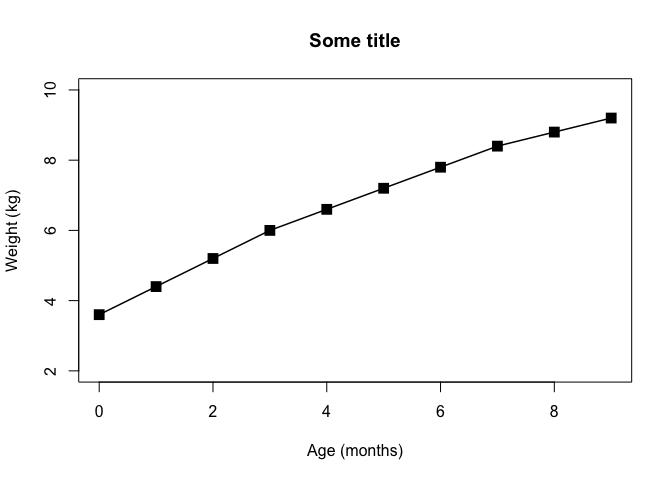
\includegraphics{Code_Generalization_files/figure-latex/unnamed-chunk-2-1.pdf}

\begin{Shaded}
\begin{Highlighting}[]
\KeywordTok{rap_pdb_forme}\NormalTok{(}\StringTok{"1AKE"}\NormalTok{)}
\end{Highlighting}
\end{Shaded}

\begin{verbatim}
##   Note: Accessing on-line PDB file
\end{verbatim}

\begin{verbatim}
## Warning in get.pdb(file, path = tempdir(), verbose = FALSE): /var/folders/
## 36/h1nlfl81237009k9zbnc0y6c0000gn/T//RtmplWnkCK/1AKE.pdb exists. Skipping
## download
\end{verbatim}

\begin{verbatim}
##    PDB has ALT records, taking A only, rm.alt=TRUE
\end{verbatim}

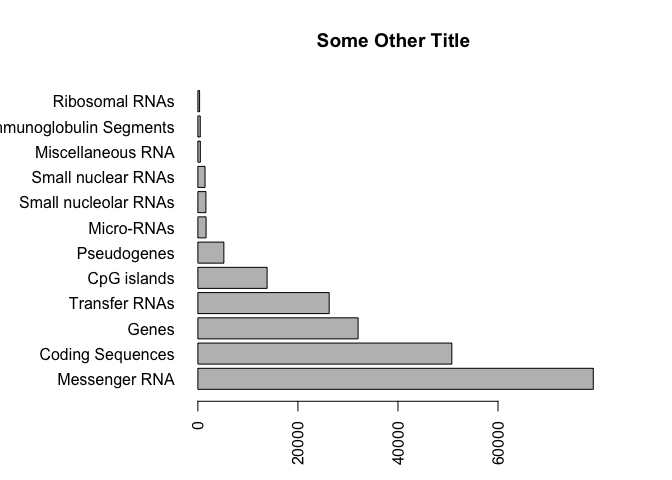
\includegraphics{Code_Generalization_files/figure-latex/unnamed-chunk-2-2.pdf}

\begin{Shaded}
\begin{Highlighting}[]
\KeywordTok{rap_pdb_forme}\NormalTok{(}\StringTok{"1E4Y"}\NormalTok{)}
\end{Highlighting}
\end{Shaded}

\begin{verbatim}
##   Note: Accessing on-line PDB file
\end{verbatim}

\begin{verbatim}
## Warning in get.pdb(file, path = tempdir(), verbose = FALSE): /var/folders/
## 36/h1nlfl81237009k9zbnc0y6c0000gn/T//RtmplWnkCK/1E4Y.pdb exists. Skipping
## download
\end{verbatim}

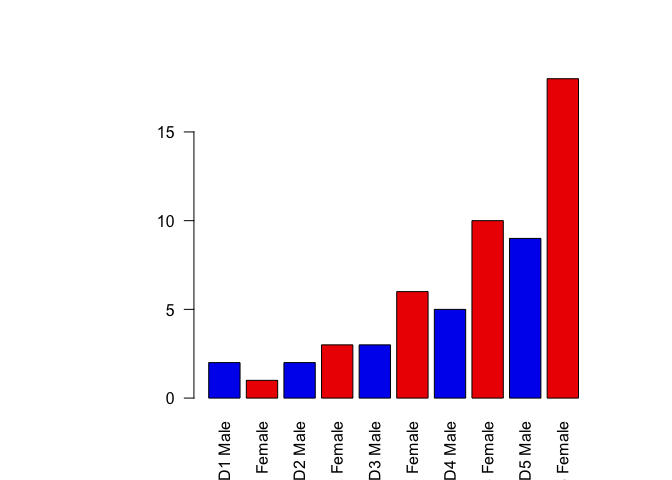
\includegraphics{Code_Generalization_files/figure-latex/unnamed-chunk-2-3.pdf}


\end{document}
